\documentclass[11pt,a4paper]{article}
\usepackage[utf8x]{inputenc}
\usepackage[T1]{fontenc}
\usepackage{graphicx}
\usepackage[usenames, dvipsnames]{color}
\usepackage{fancyhdr}
\usepackage{datetime}
\setlength{\headheight}{15.2pt}
\pagestyle{fancy}
\fancyhf{}

\lhead{\textbf{\Large\color{MidnightBlue}Design and Modelling of Software Systems 
    \hfill Page: \thepage \\ ETFOS, 2011}}

\setlength{\parindent}{0cm}

\begin{document}
\large
Laboration Assignment No. 4\\
Submission Date - \yyyymmdddate \today \\
Damir, Jelić, damir.jelic@etfos.hr \\
Marijan, Svalina, msvalina@etfos.hr
\\
\rule{\linewidth}{0.1mm}

\setcounter{section}{4}
\subsection{Chess class diagram}
\begin{figure}[htb]
    \begin{center}
        \setlength\fboxsep{0pt}
        \fbox{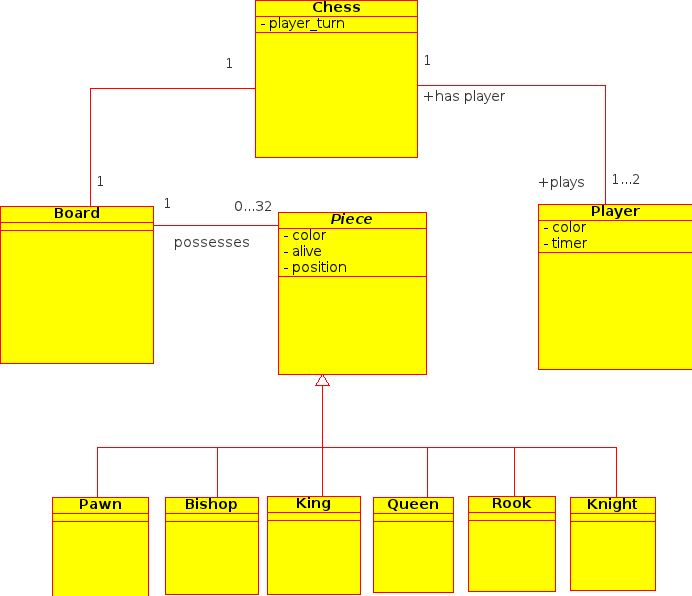
\includegraphics[scale=0.6]{class_diagram.png}}
        \caption{Chess class diagram}
        \label{fig:class_diag}
    \end{center}
\end{figure}

\begin{description}
    \item[]
    In this laboration we started with the class \emph{Chess}.
    Chess is a two player board game, so we added the 
    classes \emph{Player} and \emph{Board}.
    \item[]
    Each player has several different pieces, for each piece we created a class
    but the different pieces share some common properties so we created a general abstract class
    called \emph{Piece}. 
    \item[]
    The \emph{Chess} class only has the attribute \emph{player\_turn} which 
    remembers which player makes the next move.
    \item[]
    The class \emph{Player} has the attributes \emph{color}, which identifies
    the color the player has choosen to play with, and \emph{timer} which serves as a
    counter if the chess game is played with time control.
    \item[]
    The \emph{Piece} class has a color attribute for the color of the piece (black or white),
    the \emph{alive} attribute shows if the piece is still on the board or if the piece
    has been captured and the \emph{position} attribute which holds the current position of
    the piece on the board.
    \item[]
        The multiplicities are as follows:
        \begin{itemize}
            \item The chess game can have 1 or 2 players (eg. if one is playing against oneself)
            \item The chess game can only have 1 board
            \item The board can hold 0 to 32 pieces
        \end{itemize}
\end{description}

\end{document}
